\chapter{Grundlegende Konzepte}

Die Software unterscheidet zwischen zwei Typen von Ausgaben:

\begin{itemize}[nosep]
	\item Wiederkehrende Umsätze
	\item (Einzigartige) Umsätze
\end{itemize}

\section{Wiederkehrende Umsätze} \label{sec:fixedExpenses}

Wiederkehrende Umsätze treten in einem bestimmten Rhythmus auf (bspw. vierteljährlich oder monatlich) oder aber auch unregelmäßig, dafür aber wiederkehrend (bspw. Tanken).

\begin{figure}[ht!]
	\centering
	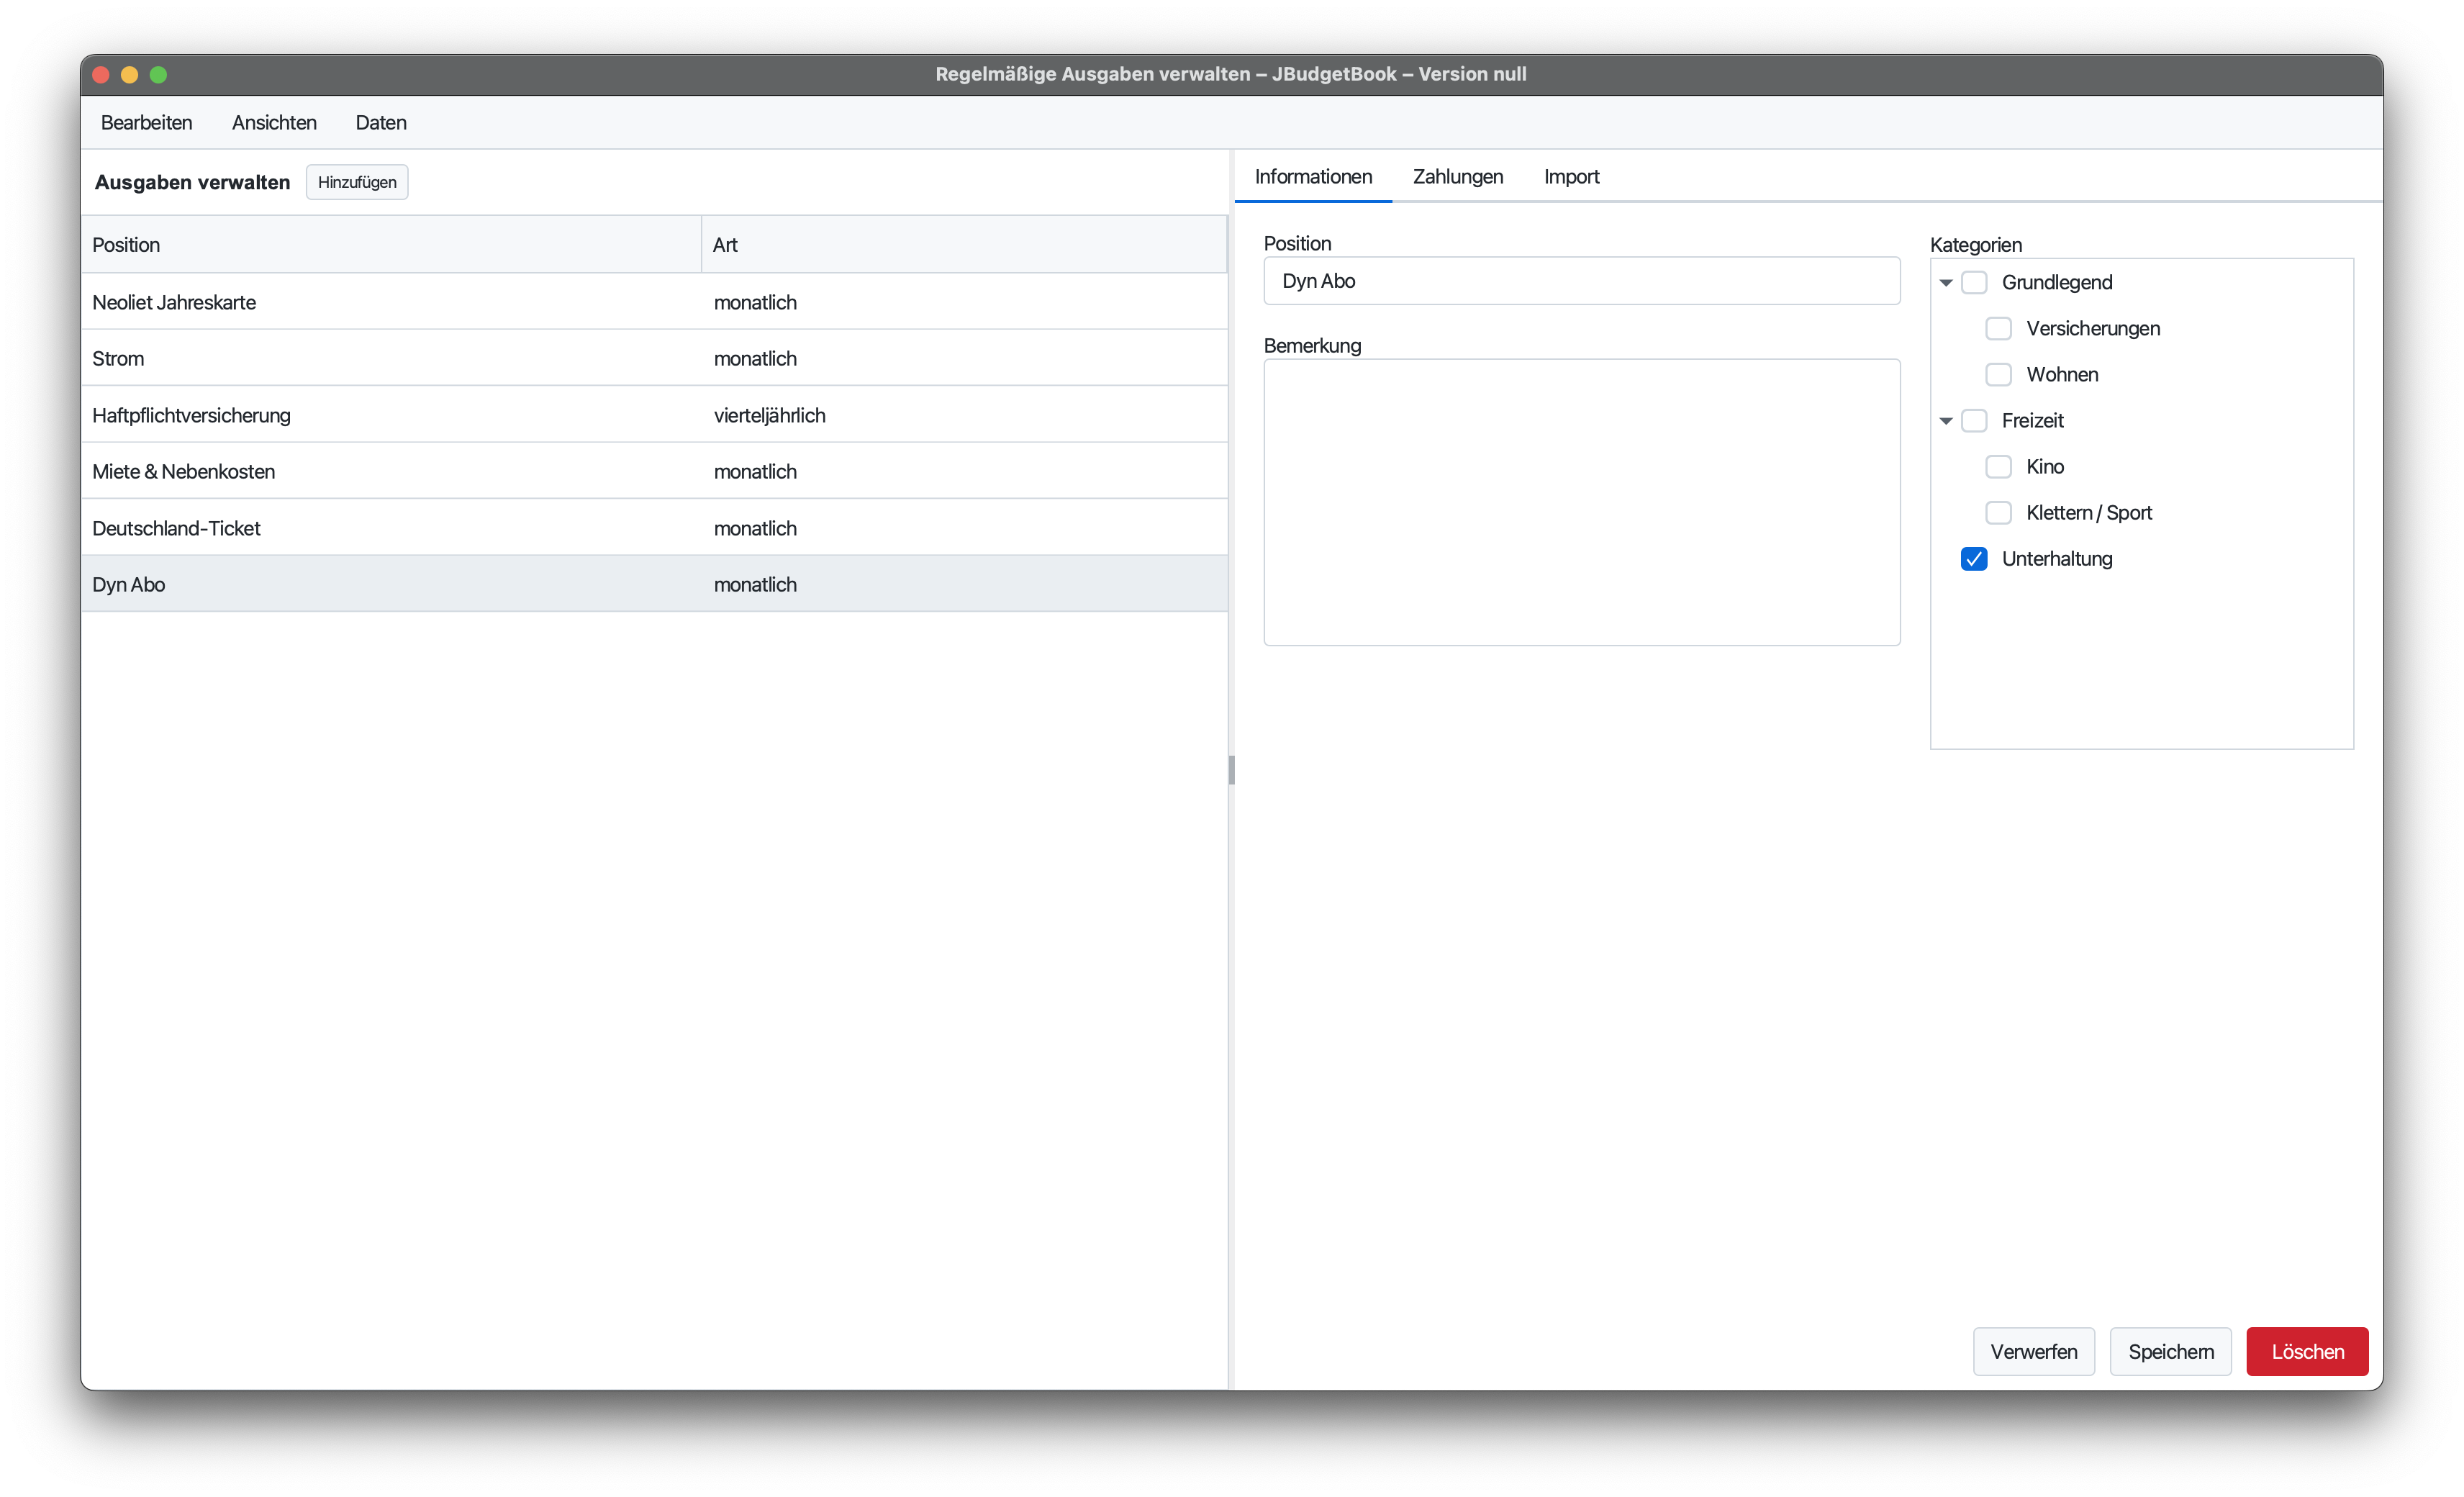
\includegraphics[width=\textwidth]{img/Screenshot-FixedExpenses-MDV}
	\vspace{-2em}
	\caption{Listen- \& Detailansicht der regelmäßigen Ausgaben}
	\label{fig:mdvFixedExpenses}
\end{figure}

In der Detailansicht (s. Abbildung \ref{fig:mdvFixedExpenses} rechts) kann u. a. der Zyklus/Rhythmus (s. "`Zahlungen"' des Umsatzes und die Importregeln festgelegt werden. Beide Angaben sind optional.

\renewcommand{\arraystretch}{1.5}
\begin{table}[!ht]
\centering
\begin{tabular}{|p{6cm}|p{8cm}|}
\hline 
\textbf{Feld} & \textbf{Beschreibung} \\ 
\hline 
Position * & Bezeichnung des Umsatzes \\ 
\hline 
Bemerkung & Anmerkung zum Umsatz \\ 
\hline 
Richtung * & Richtung (Einnahme oder Ausgabe) \\ 
\hline 
Kategorien & Kategorien, denen der Umsatz zugeordnet ist \\ 
\hline 
Zahlungen nur für die Zukunft (und den aktuellen Monat) verwenden & Wenn die Checkbox ausgewählt ist, werden die konfigurierten Zahlungen nicht für die Vergangenheit verwendet (s. Beispiel unten) \\ 
\hline 
\end{tabular} 
\caption{Konfigurationsmöglichkeiten im Tab "`Informationen"'}
\end{table}
\renewcommand{\arraystretch}{1.0}

\renewcommand{\arraystretch}{1.5}
\begin{table}[!ht]
\centering
\begin{tabular}{|p{6cm}|p{8cm}|}
\hline 
\textbf{Feld} & \textbf{Beschreibung} \\ 
\hline 
Betrag * & Höhe des Umsatzes \\ 
\hline 
Art * & Rhythmus des Umsatzes (monatlich, vierteljährlich, halbjährlich, jährlich) \\ 
\hline 
Von * & Bspw. ab wann der Umsatz in dieser Höhe ansteht \\ 
\hline 
Bis & Bspw. bis wann der Umsatz in dieser Höhe ansteht (kann leer gelassen werden, wenn der Umsatz aktuell in dieser Höhe ansteht) \\ 
\hline 
\multicolumn{2}{|p{14cm}|}{In der Tabelle können mehrere "`Zahlungen"' hinterlegt werden. Das ermöglicht die Abbildung von steigenden oder sinkenden Umsätzen, wie es bspw. bei Versicherungsbeiträgen häufig der Fall ist.} \\ 
\hline 
\end{tabular} 
\caption{Konfigurationsmöglichkeiten im Tab "`Zahlungen"'}
\end{table}
\renewcommand{\arraystretch}{1.0}

\renewcommand{\arraystretch}{1.5}
\begin{table}[!ht]
\centering
\begin{tabular}{|p{6cm}|p{8cm}|}
\hline 
\textbf{Feld} & \textbf{Beschreibung} \\ 
\hline 
Tabelle "`Importregeln"' & Diese Tabelle ermöglicht die Verwaltung einer Liste an Importregeln (s. Kapitel \ref{chap:import}) \\ 
\hline 
Tabelle "`Zugeordnete Importe"' & Listet alle zugeordneten Importe auf (readonly) \\ 
\hline 
\end{tabular} 
\caption{Konfigurationsmöglichkeiten im Tab "`Import"'}
\end{table}
\renewcommand{\arraystretch}{1.0}

\begin{infobox}
\textbf{Hinweis zu importieren Umsätzen}: Sollten zu einer Ausgabe reale Umsätze importiert worden sein, werden in den Übersichten (bspw. Monatsansicht) der Betrag dieser importierten Umsätze verwendet und der im System konfigurierte Betrag nur noch als Fallback verwendet. Eine detailliertere Beschreibung findet sich in Kapitel \ref{chap:import}. 
\end{infobox}

Da reale Ausgaben (bzw. Importe) über die Importregeln einer regelmäßigen Ausgabe zugeordnet werden können und dann dieser reale Umsatz in der Software angezeigt wird, können auch wiederkehrende Ausgaben mit schwankenden Beträgen -- wie es beim Tanken der Fall ist -- gruppiert werden.

\subsection*{Beispiel: Tanken}

Die Ausgabe "`Tanken"' soll als wiederkehrender Umsatz (Richtung "`Ausgabe`"') im System abgebildet werden. Dazu kann eine "`Zahlung"' in der Höhe von bspw. 80 Euro monatlich angelegt werden. Allerdings wird nicht jeden Monat getankt, weshalb die Checkbox "`Zahlungen nur für die Zukunft (und den aktuellen Monat) verwenden"' ausgewählt wird. Somit werden bspw. in der Analyseansicht für vergangene Monate die realen Ausgaben angezeigt -- wie sie vom Konto importiert wurden --, während für die Zukunft weiterhin die geplanten Zahlungen aufgeführt werden. Wenn man regelmäßig an einer Star- oder Aral-Tankstelle tankt und mittels Visa-Karte bezahlt, könnten zwei Importregeln konfiguriert werden, die jeweils  "`VISA STAR"' und "`VISA ARAL"' als "`Empfänger enthält"' eingetragen haben. 

Sollte das Import-Feature nicht genutzt werden, kann ein "`realer Umsatz"' auch manuell als (einzigartiger) Umsatz (bzw. Ausgabe) konfiguriert und mit der wiederkehrenden Ausgabe "`Tanken"' verknüpft werden. Dann wird für den entsprechenden Monat ebenfalls der gesamte Betrag dieser Ausgabe verwendet, statt der geplanten Zahlung der wiederkehrenden Ausgabe.


\section{Einzigartige Ausgaben}

Einzigartige Ausgaben bzw. einmalige Ausgaben treten einmalig oder selten auf, sodass es keinen Mehrwert bietet, diese als regelmäßige Ausgaben zu gruppieren (da bspw. keine wiederkehrende Importe zu Ausgaben dieser Art erwartet werden).

\section{Datenmodell} 

\begin{figure}[ht!]
	\centering
	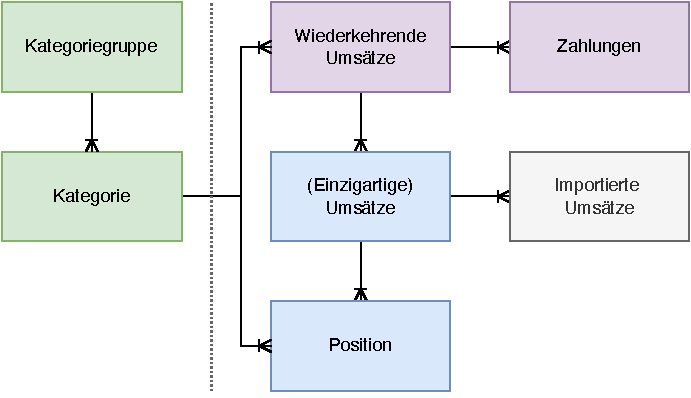
\includegraphics[width=.8\textwidth]{img/DataModel}
	\vspace{0em}
	\caption{Datenmodell}
	\label{fig:datamodel}
\end{figure}